% ----------------------------------------------------------
\chapter{Introdução}\label{cap:intro}
% ----------------------------------------------------------

Desde a criação do padrão CubeSat em 1999, nanossatélites tem sido utilizados em cada vez mais aplicações. Popularizado inicialmente no meio acadêmico, possibilitando à universidades o desenvolvimento de missões espaciais de baixo custo, atualmente estes satélites são utilizados para diversas aplicações, como mostrado em \textcite{modern-small-sats-economics}.

Inicialmente os CubeSats serviam um propósito didático, com aplicações de demonstração de tecnologia, experimentos científicos.
Porém, recentemente, aplicações comerciais de nanossatélites e CubeSats tem ganhado espaço, relata \textcite{modern-small-sats-economics} tanto que em 2014 o numero de lançamentos de nanossatélites com propósito comercial ultrapassou os de propósito acadêmico.

Com o advento de conceitos como “\textit{New Space}” e a percepção de sua utilidade comercial, os pequenos satélites estão entrando no radar de grandes empresas, com SpaceX e Boeing, planejando a utilização de grandes constelações, conforme observado por \textcite{modern-small-sats-economics}.
Inclusive, CubeSats vem sendo utilizados em pesquisas e missões espaciais de alto nível, com grandes instituições como a NASA em seu programa Artemis, mostrado em \textcite{artemis-plan}, que utilizará de CubeSats em sua missão com o objetivo de explorar a lua.

% ----------------------------------------------------------
\section{Falhas em CubeSats}\label{sec:intro-falhas}
% ----------------------------------------------------------

Com a proposta de baixo custo, rápido desenvolvimento e uso de componentes \gls{COTS}, a confiabilidade dos CubeSats foi significativamente reduzida em relação à satélites de grande porte, que utilizam componentes robustos desenvolvidos especificamente para aplicações espaciais e passam por processos rigorosos de testes, validação e qualificação.
Como consequência disso, observaram-se grandes taxas de falhas em missões de CubeSats.

Conforme \textcite{survey-nanosat-missions-2010}, até 2010, cerca de 32\% dos lançamentos de nanossatélites resultaram em falha, e considerando apenas os lançamentos bem sucedidos, apenas cerca de 48\% das missões tiveram sucesso total.

O estudo de \textcite{first-100-cubesats}, similarmente aponta taxas de falha de aproximadamente 50\% em missões acadêmicas de CubeSat.
Também neste estudo, esta alta taxa é atribuída a uma carência de testes funcionais a nível de integração dos satélites, visto que, em missões acadêmicas, devido a cronogramas justos ou orçamentos limitados, costuma-se realizar apenas os testes ambientais requeridos para lançamento.
Segundo o autor, estes testes são fundamentais para identificar possíveis falhas na operação do satélite.

No trabalho de \textcite{reliability-of-cubesats}, que analisou a causa de falha de diversos CubeSats lançados até 2014, aponta-se o \gls{EPS} como principal módulo causador de falhas em CubeSats.

Para satélites de propósito educacional, de demonstração tecnológica, essa baixa confiabilidade é tolerável, visto que parte do objetivo destas missões inclui proporcionar experiência e capacitação para estudantes.
Porém, é inaceitável para aplicações comerciais \cite{overview-nanosat-test}.

Esta taxa de falha, no entanto, vem diminuindo desde então, com com uma taxa de apenas 10\% de falhas em lançamentos em 2018 segundo \textcite{aiv-istsat-1}. Conforme a base de dados de nanossatélites Nanosats Database, de \textcite{nanosats-database}, observando a situação dos nanossatélites lançados até dezembro de 2023, mostrados na \autoref{fig:status-nanosats}, tem-se aproximadamente 5\% dos satélites com falhas no lançamento. Ainda, satélites não-operacionais constituem apenas 21\%, aproximadamente, considerando-se os satélites classificados em operacionais ou não-operacionais.
O aumento no número de aplicações comerciais, desenvolvidas por equipes mais experientes e com mais recursos, é um dos fatores que tem contribuído para essa mudança.
Outro fator importante, como relatado em \textcite{aiv-istsat-1}, missões acadêmicas tem dado maior atenção aos processos de \gls{AIV}.

\begin{figure}[htp]
    \caption{Estado atual dos nanossatélites lançados (dezembro de 2023).}
    \begin{center}
        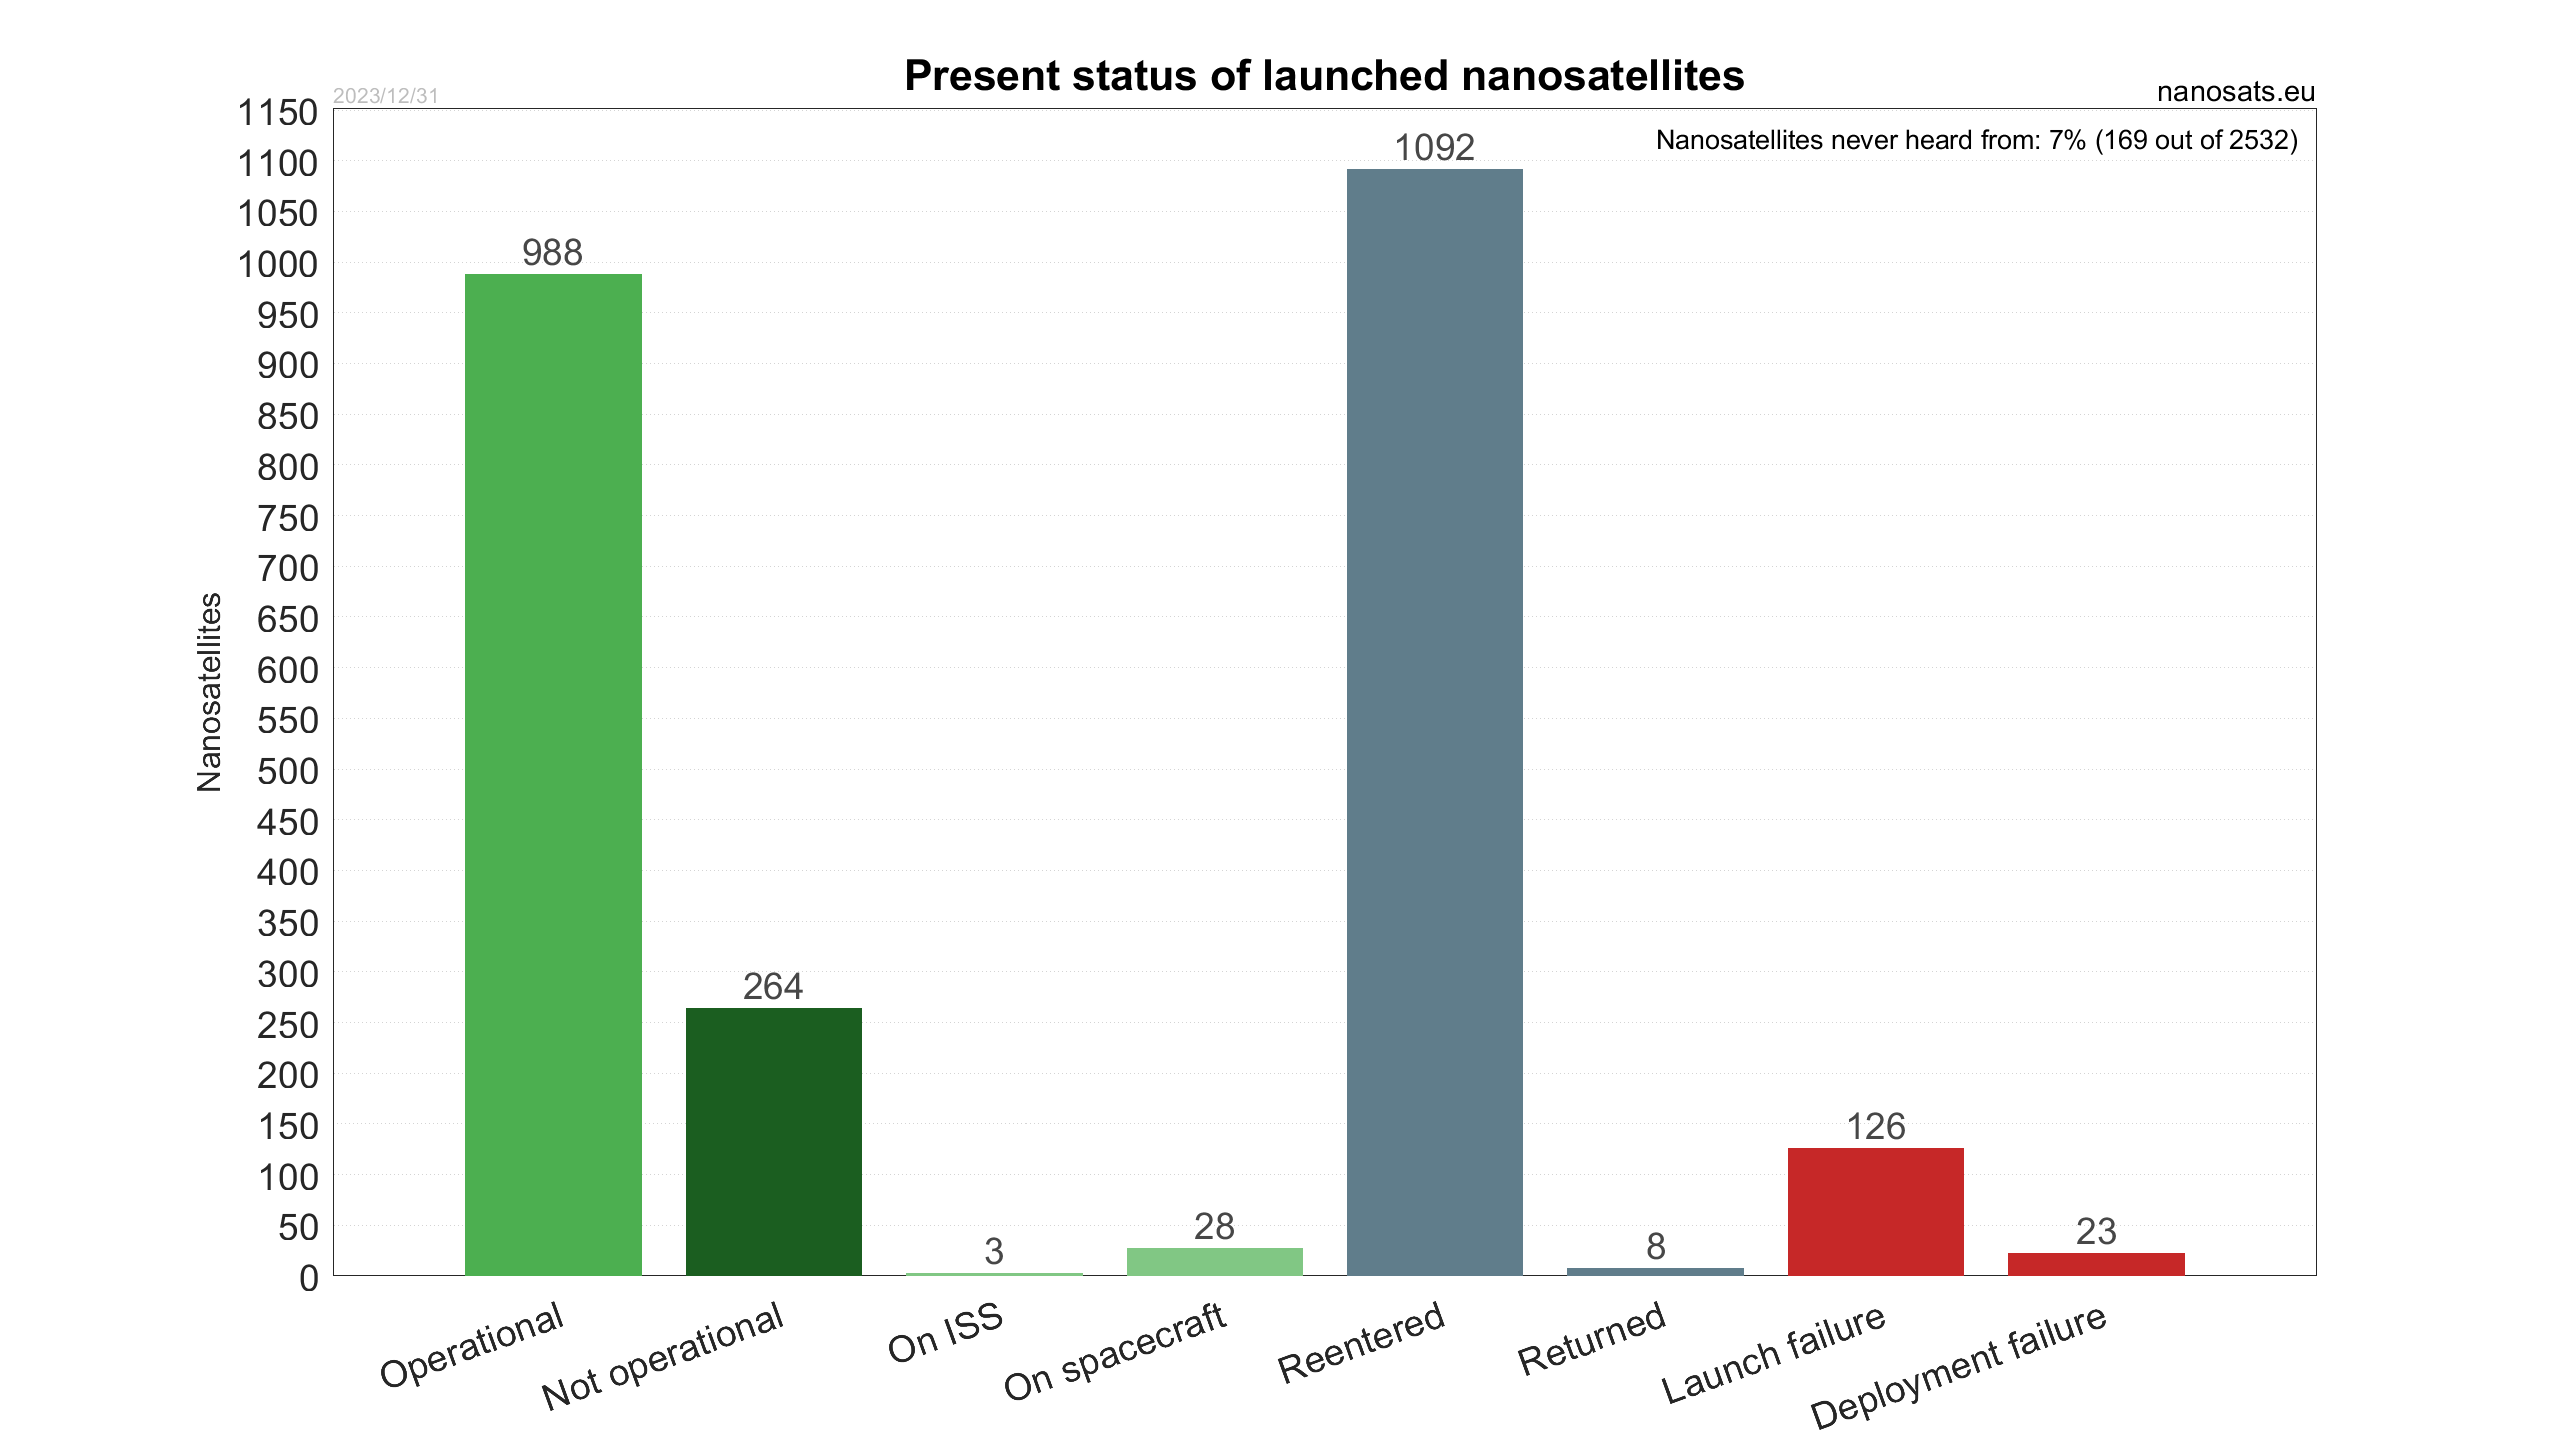
\includegraphics[width=\textwidth, keepaspectratio]{images/Nanosats_status_2023-12-31_large.png}
    \end{center}
    \fonte{\textcite{nanosats-database}.}
    \label{fig:status-nanosats}
\end{figure}


Nota-se também que, em missões de CubeSats mais recentes, foram adotados procedimentos e padrões mais rigorosos, não só em relação à testes, mas em todo o processo de engenharia de sistemas e gerenciamento da missão.
Trabalhos como \textcite{floripasat-1} e \textcite{tailoring-ecss-nanosat}, por exemplo, tomaram como referência os padrões determinados pela \gls{ECSS}, utilizados pela \gls{ESA} e diversas outras agências espaciais da Europa.

% ----------------------------------------------------------
\section{Projetos do SpaceLab}\label{sec:intro-spacelab}
% ----------------------------------------------------------

O FloripaSat-1, descrito em \textcite{floripasat-1}, foi o primeiro CubeSat desenvolvido e lançado pelo Laboratório de Pesquisa em Sistemas Espaciais da UFSC, o SpaceLab, com uma missão de demonstração tecnológica de sua plataforma de serviço multi-missão totalmente desenvolvida por estudantes da \gls{UFSC}.

A plataforma de serviço FloripaSat consiste de três módulos principais, \gls{OBDH}, responsável pelo controle e gerenciamento de dados, \gls{TTC}, responsável pela comunicação com as estações terrestres e recepção de telecomandos, e \gls{EPS}, responsável pela coleta, armazenamento e distribuição de energia.

Após o lançamento do FloripaSat-1, o SpaceLab continuou desenvolvendo e aprimorando sua plataforma de serviço para futuras missões, resultando no desenvolvimento da segunda geração de módulos, que em conjunto formam a plataforma FloripaSat-2 \cite{floripasat2}.

O \gls{EPS2} é a segunda geração de módulo \gls{EPS} desenvolvido para a plataforma multi-missão do laboratório, será utilizado nas missões GOLDS-UFSC e Constelação Catarina e encontra-se nos estágios finais de desenvolvimento. Este \gls{EPS} é uma evolução direta do módulo utilizado no FloripaSat-1, seguindo a mesma arquitetura, porém, aplicando as lições aprendidas com o primeiro lançamento.

Visto que o \gls{EPS} é o principal causador de falhas em CubeSats, iniciou-se também no laboratório a concepção do \gls{REEPS}, com o objetivo de desenvolver um módulo de \gls{EPS} de alta confiabilidade e robustez.

No momento da escrita deste trabalho, o primeiro modelo de engenharia do \gls{REEPS} está em processo de fabricação.
Também, a terceira geração de módulos para a plataforma multi-missão está em fase inicial de desenvolvimento, o que implicará no design de ainda mais um modelo de \gls{EPS} feito no SpaceLab.

Com diferentes projetos, em diferentes estágios de desenvolvimento e diferentes arquiteturas de \gls{EPS} sendo utilizadas nas missões do laboratório, percebeu-se a necessidade de aprimorar os procedimentos de teste utilizados, especialmente na etapa de qualificação, assim como a necessidade de avaliar a performance dos diferentes módulos de \gls{EPS}.

% ----------------------------------------------------------
\section{Motivação}\label{sec:intro-motivacao}
% ----------------------------------------------------------

Como observado anteriormente, processos de \gls{AIV} mais rigorosos, seguindo padrões como \gls{ECSS} adaptados para o cenário de um nanossatélite, tem sido aplicados em missões envolvendo CubeSats, mais especificamente, na etapa de qualificação do satélite como um todo.
Porém, tratando-se dos módulos individualmente, especificamente módulos de EPS, não se observam os mesmos cuidados e estruturação nos procedimentos de teste e a adoção desses padrões, quando mencionados, como em \textcite{mist-eps}, ainda é de forma bastante simplificada.

Neste contexto, propõe-se então a elaboração de um documento contendo diretrizes e orientações acerca da elaboração de planos de testes para módulos \gls{EPS}, baseado nos padrões da \gls{ECSS}, adaptável para diferentes topologias e arquiteturas, a ser utilizado pela equipe do SpaceLab.

Este trabalho consistira na realização de uma revisão de topologias e arquiteturas de EPSs para CubeSats, bem como de campanhas de teste executadas nestes módulos, seguida por uma análise das normas ECSS-E-ST-10-02 \cite{ecss-e-st-10-02} e ECSS-E-ST-10-03 \cite{ecss-e-st-10-03} relacionadas ao processo de verificação e testes. A partir destas analises, será elaborado um documento contento uma série de diretrizes e orientações para a elaboração de planos de testes voltado para EPSs de CubeSats. Por fim, como demonstração, será elaborado um plano de testes simplificado para o \gls{EPS2}, seguindo as orientações propostas.

% ----------------------------------------------------------
\section{Objetivos}\label{sec:objetivos}
% ----------------------------------------------------------

Nas seções abaixo estão descritos o objetivo geral e os objetivos específicos deste trabalho.

% ----------------------------------------------------------
\subsection{Objetivo Geral}
% ----------------------------------------------------------

% Propor uma estrutura de plano de testes aplicável à diferentes topologias de módulos de \gls{EPS}s de CubeSats baseado nos padrões da \gls{ECSS}.

Elaboração de um documento contendo diretrizes e orientações para preparação de planos de teste para módulos \gls{EPS}, baseado nas normas e padrões da \gls{ECSS}, de forma que o mesmo seja aplicável à diferentes topologias e arquiteturas.

% ----------------------------------------------------------
\subsection{Objetivos Específicos}
% ----------------------------------------------------------

\begin{itemize}
    \item Analisar as normas da ECSS relacionadas a procedimentos de teste.
    \item Identificar os principais blocos de teste necessários.
    \item Identificar as principais funções e características de um \gls{EPS} a serem testadas.
    \item Propor uma estrutura de documentação para os testes.
    \item Desenvolver um plano de testes para o \gls{EPS2} baseado na proposta deste trabalho.
\end{itemize}